%% LyX 2.0.5.1 created this file.  For more info, see http://www.lyx.org/.
%% Do not edit unless you really know what you are doing.
\documentclass{article}\usepackage{graphicx, color}
%% maxwidth is the original width if it is less than linewidth
%% otherwise use linewidth (to make sure the graphics do not exceed the margin)
\makeatletter
\def\maxwidth{ %
  \ifdim\Gin@nat@width>\linewidth
    \linewidth
  \else
    \Gin@nat@width
  \fi
}
\makeatother

\IfFileExists{upquote.sty}{\usepackage{upquote}}{}
\definecolor{fgcolor}{rgb}{0.2, 0.2, 0.2}
\newcommand{\hlnumber}[1]{\textcolor[rgb]{0,0,0}{#1}}%
\newcommand{\hlfunctioncall}[1]{\textcolor[rgb]{0.501960784313725,0,0.329411764705882}{\textbf{#1}}}%
\newcommand{\hlstring}[1]{\textcolor[rgb]{0.6,0.6,1}{#1}}%
\newcommand{\hlkeyword}[1]{\textcolor[rgb]{0,0,0}{\textbf{#1}}}%
\newcommand{\hlargument}[1]{\textcolor[rgb]{0.690196078431373,0.250980392156863,0.0196078431372549}{#1}}%
\newcommand{\hlcomment}[1]{\textcolor[rgb]{0.180392156862745,0.6,0.341176470588235}{#1}}%
\newcommand{\hlroxygencomment}[1]{\textcolor[rgb]{0.43921568627451,0.47843137254902,0.701960784313725}{#1}}%
\newcommand{\hlformalargs}[1]{\textcolor[rgb]{0.690196078431373,0.250980392156863,0.0196078431372549}{#1}}%
\newcommand{\hleqformalargs}[1]{\textcolor[rgb]{0.690196078431373,0.250980392156863,0.0196078431372549}{#1}}%
\newcommand{\hlassignement}[1]{\textcolor[rgb]{0,0,0}{\textbf{#1}}}%
\newcommand{\hlpackage}[1]{\textcolor[rgb]{0.588235294117647,0.709803921568627,0.145098039215686}{#1}}%
\newcommand{\hlslot}[1]{\textit{#1}}%
\newcommand{\hlsymbol}[1]{\textcolor[rgb]{0,0,0}{#1}}%
\newcommand{\hlprompt}[1]{\textcolor[rgb]{0.2,0.2,0.2}{#1}}%

\usepackage{framed}
\makeatletter
\newenvironment{kframe}{%
 \def\at@end@of@kframe{}%
 \ifinner\ifhmode%
  \def\at@end@of@kframe{\end{minipage}}%
  \begin{minipage}{\columnwidth}%
 \fi\fi%
 \def\FrameCommand##1{\hskip\@totalleftmargin \hskip-\fboxsep
 \colorbox{shadecolor}{##1}\hskip-\fboxsep
     % There is no \\@totalrightmargin, so:
     \hskip-\linewidth \hskip-\@totalleftmargin \hskip\columnwidth}%
 \MakeFramed {\advance\hsize-\width
   \@totalleftmargin\z@ \linewidth\hsize
   \@setminipage}}%
 {\par\unskip\endMakeFramed%
 \at@end@of@kframe}
\makeatother

\definecolor{shadecolor}{rgb}{.97, .97, .97}
\definecolor{messagecolor}{rgb}{0, 0, 0}
\definecolor{warningcolor}{rgb}{1, 0, 1}
\definecolor{errorcolor}{rgb}{1, 0, 0}
\newenvironment{knitrout}{}{} % an empty environment to be redefined in TeX

\usepackage{alltt}
\usepackage[sc]{mathpazo}
\usepackage{geometry}
\geometry{verbose,tmargin=2.5cm,bmargin=2.5cm,lmargin=2.5cm,rmargin=2.5cm}
\setcounter{secnumdepth}{2}
\setcounter{tocdepth}{2}
\usepackage{url}
\usepackage[unicode=true,pdfusetitle,
 bookmarks=true,bookmarksnumbered=true,bookmarksopen=true,bookmarksopenlevel=2,
 breaklinks=false,pdfborder={0 0 1},backref=false,colorlinks=false]
 {hyperref}
\hypersetup{
 pdfstartview={XYZ null null 1}}
\usepackage{breakurl}
\begin{document}





\title{Stat 2025- HW 2}
\author{Michael Discenza}

\maketitle

\section{Best-subset Model Selection using Cross-validation}
I first load the library that will help with the cross-validation and then I import houseprice dataset into R
\begin{knitrout}
\definecolor{shadecolor}{rgb}{0.969, 0.969, 0.969}\color{fgcolor}\begin{kframe}
\begin{alltt}
\hlfunctioncall{library}(DAAG)
houseprices <- \hlfunctioncall{read.delim}(\hlstring{"http://www.stat.columbia.edu/~madigan/W2025/data/houseprices.txt"})
\end{alltt}
\end{kframe}
\end{knitrout}


Next, I define two helper functions. The first, which is based on the source from Hadley Wickham's Meify Package (see \url{https://github.com/hadley/meifly/blob/master/R/generate.r}) returns all possible simple linear models that can be made from the set of predictors:


\begin{knitrout}
\definecolor{shadecolor}{rgb}{0.969, 0.969, 0.969}\color{fgcolor}\begin{kframe}
\begin{alltt}
all_possible_models <- \hlfunctioncall{function}(x.column.names, y.col.name) \{
    Cols <- x.column.names
    n <- \hlfunctioncall{length}(Cols)
    id <- \hlfunctioncall{unlist}(\hlfunctioncall{lapply}(1:n, \hlfunctioncall{function}(i) \hlfunctioncall{combn}(1:n, i, simplify = F)), recursive = F)
    Formulas <- \hlfunctioncall{sapply}(id, \hlfunctioncall{function}(i) \hlfunctioncall{paste}(y.col.name, \hlstring{"~"}, \hlfunctioncall{paste}(Cols[i], collapse = \hlstring{"+"})))
\}
\end{alltt}
\end{kframe}
\end{knitrout}



The second function does five-fold cross vaidation on the data set for a given model (formula) input and returns the cross-validated means squared error:
\begin{knitrout}
\definecolor{shadecolor}{rgb}{0.969, 0.969, 0.969}\color{fgcolor}\begin{kframe}
\begin{alltt}
apply_formula <- \hlfunctioncall{function}(model, cv = 5) \{
\hlcomment{    #make the default value for this function 5}
    cv.model <- \hlfunctioncall{CVlm}(houseprices, \hlfunctioncall{lm}(model, data = houseprices), m = cv)
    cvmse <- \hlfunctioncall{mean}(\hlfunctioncall{abs}(cv.model$sale.price - cv.model$cvpred))
\}
\end{alltt}
\end{kframe}
\end{knitrout}


I then combine these functions to return the cross-validated mean squared error for the all of the possible simple linear models:
\begin{knitrout}
\definecolor{shadecolor}{rgb}{0.969, 0.969, 0.969}\color{fgcolor}\begin{kframe}
\begin{alltt}
FORMULAS <- \hlfunctioncall{all_possible_models}(x.column.names = \hlfunctioncall{colnames}(houseprices[1:3]), y.col.name = \hlfunctioncall{colnames}(houseprices[4]))
CV.MSE <- \hlfunctioncall{lapply}(FORMULAS, apply_formula)
final.results <- \hlfunctioncall{cbind}(FORMULAS, CV.MSE)
\end{alltt}
\end{kframe}
\end{knitrout}


\begin{knitrout}
\definecolor{shadecolor}{rgb}{0.969, 0.969, 0.969}\color{fgcolor}\begin{kframe}
\begin{alltt}
final.results
\end{alltt}
\begin{verbatim}
##      FORMULAS                            CV.MSE
## [1,] "sale.price ~ floors"               43.2  
## [2,] "sale.price ~ area"                 46.4  
## [3,] "sale.price ~ bedrooms"             34.2  
## [4,] "sale.price ~ floors+area"          47.7  
## [5,] "sale.price ~ floors+bedrooms"      35.4  
## [6,] "sale.price ~ area+bedrooms"        27.6  
## [7,] "sale.price ~ floors+area+bedrooms" 28.1
\end{verbatim}
\end{kframe}
\end{knitrout}


Comparing the cross-validated mean squared errors for each model, we can see that the best simple linear model is sale.price ~ floors+area+bedrooms.  A summary of this model is shown below:
\begin{knitrout}
\definecolor{shadecolor}{rgb}{0.969, 0.969, 0.969}\color{fgcolor}\begin{kframe}
\begin{alltt}
lm.optimatal <- \hlfunctioncall{lm}(sale.price ~ area + bedrooms, data = houseprices)
\hlfunctioncall{summary}(lm.optimatal)
\end{alltt}
\begin{verbatim}
## 
## Call:
## lm(formula = sale.price ~ area + bedrooms, data = houseprices)
## 
## Residuals:
##    Min     1Q Median     3Q    Max 
## -80.90  -4.25   1.54  13.25  42.03 
## 
## Coefficients:
##             Estimate Std. Error t value Pr(>|t|)   
## (Intercept) -141.761     67.872   -2.09   0.0587 . 
## area           0.142      0.047    3.03   0.0104 * 
## bedrooms      58.324     14.760    3.95   0.0019 **
## ---
## Signif. codes:  0 '***' 0.001 '**' 0.01 '*' 0.05 '.' 0.1 ' ' 1 
## 
## Residual standard error: 33.1 on 12 degrees of freedom
## Multiple R-squared: 0.731,	Adjusted R-squared: 0.686 
## F-statistic: 16.3 on 2 and 12 DF,  p-value: 0.000379
\end{verbatim}
\end{kframe}
\end{knitrout}

\pagebreak
\section{Checking Assumptions for Linear Regression}
First we check for to see that we were correct in assuming that the relationship is linear. One test we can conduct is plotting our our observed values for sale price against our predicted values for sale price.  Here we see that the points seem fairly randomoly distributed around the line through the diagonal so we can accept the linearity assumption. Another test for linearity is plotting residuals versus our preidcted values.  Below, this plot, the one to the right, is really only a rotation of the plot on the left. It seems as though there is slightly more of a pattern than we might have been able to visually identify before.  This casts some doubt on our linearity assumption.
\begin{knitrout}
\definecolor{shadecolor}{rgb}{0.969, 0.969, 0.969}\color{fgcolor}

{\centering 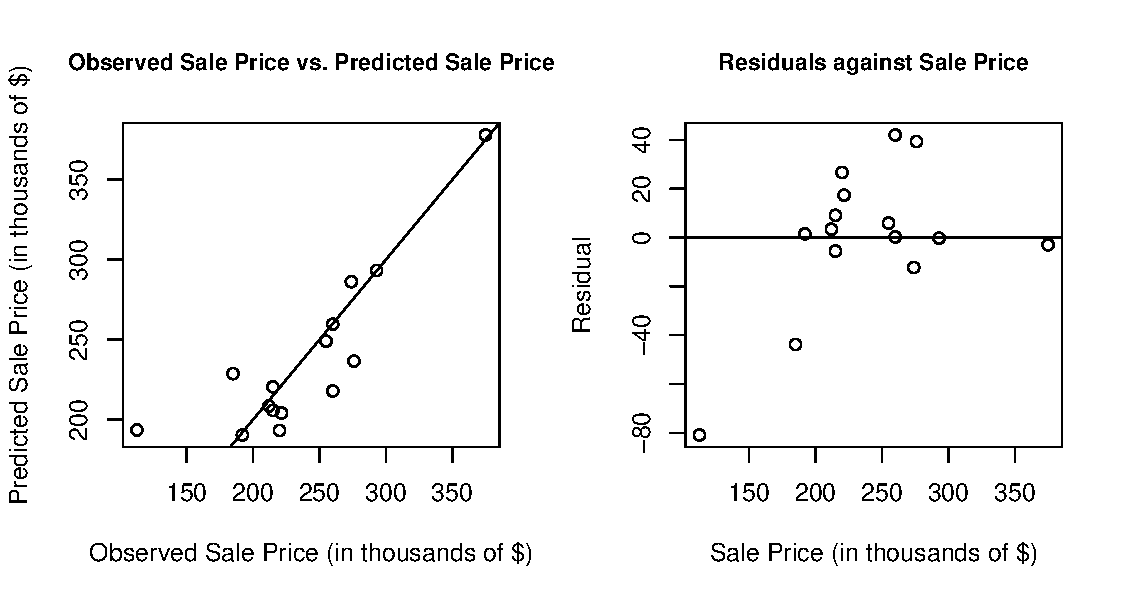
\includegraphics[width=\maxwidth]{figure/minimal-modelAssumptions1} 

}



\end{knitrout}



\pagebreak
An additional assumption that we need to check is homoscedasticity, the constant variance of home sale prices across different values of home area and number of bedrooms.  Below, it seems that in larger houses there is less variance around the fitted values.  This, however, is due to the fact that these larger houses are influential points, which have the effect of pulling the line through (or at least closely around) themselves. Ideally, there would be more houses throughout the range of the variables so that the relationships we identified are not merely the product of a few extreme data points.
\begin{knitrout}
\definecolor{shadecolor}{rgb}{0.969, 0.969, 0.969}\color{fgcolor}

{\centering 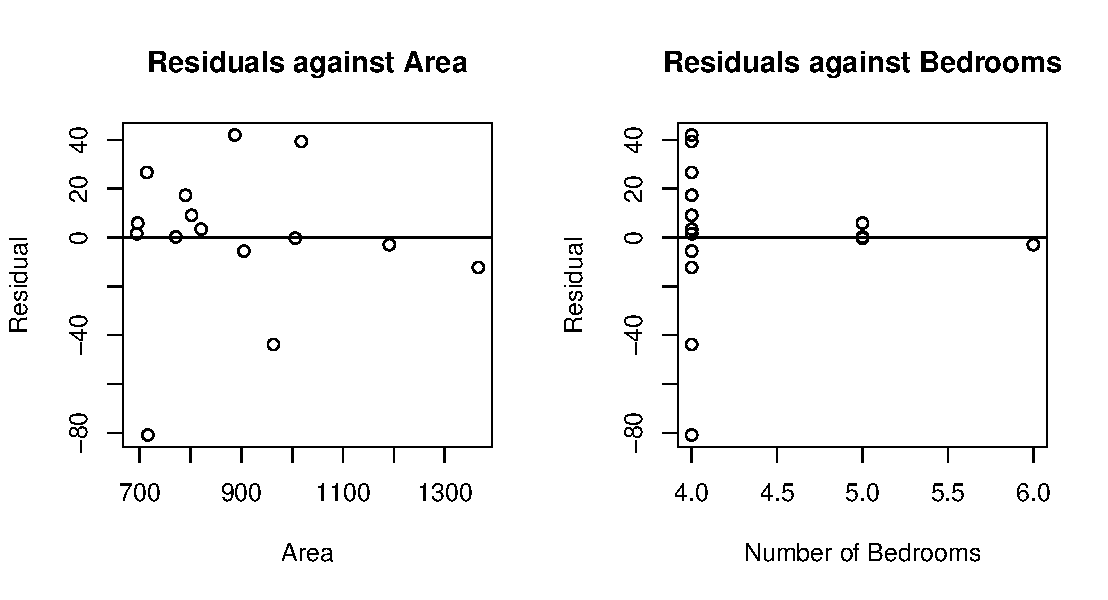
\includegraphics[width=\maxwidth]{figure/minimal-modelAssumptions3} 

}



\end{knitrout}

Finally, we test the assumption that residuals are noramlly distributed about the fitted regression line.  To analyze this relationship visually, we examine a "qqnorm" plot, which helps us compare the distribution of the scaled residuals to that of the standard normal distribution.  On the tails, there seems to be significant deviation from the normal distribution.
\begin{knitrout}
\definecolor{shadecolor}{rgb}{0.969, 0.969, 0.969}\color{fgcolor}

{\centering 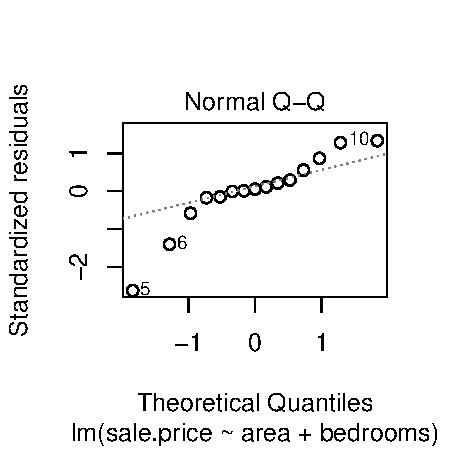
\includegraphics[width=\maxwidth]{figure/minimal-modelAssumptions2} 

}



\end{knitrout}


\pagebreak
\section{Confidence Interval for the Average Home Price}
\begin{knitrout}
\definecolor{shadecolor}{rgb}{0.969, 0.969, 0.969}\color{fgcolor}\begin{kframe}
\begin{alltt}
nd <- \hlfunctioncall{data.frame}(floors = 2, area = 1000, bedrooms = 4)
confidence_interval <- \hlfunctioncall{predict}(lm.optimatal, interval = \hlstring{"confidence"}, newdata = nd, level = 0.95)
confidence_interval
\end{alltt}
\begin{verbatim}
##   fit lwr upr
## 1 234 209 260
\end{verbatim}
\end{kframe}
\end{knitrout}

The confidence interval for the average price of two-floor, 1000 square foot house with 4 bedrooms is (209, 260), centered around 234.

\section{Prediction Interval for a Home's Price}
\begin{knitrout}
\definecolor{shadecolor}{rgb}{0.969, 0.969, 0.969}\color{fgcolor}\begin{kframe}
\begin{alltt}
nd <- \hlfunctioncall{data.frame}(floors = 2, area = 1000, bedrooms = 4)
prediction_interval <- \hlfunctioncall{predict}(lm.optimatal, interval = \hlstring{"prediction"}, newdata = nd, level = 0.95)
prediction_interval
\end{alltt}
\begin{verbatim}
##   fit lwr upr
## 1 234 158 310
\end{verbatim}
\end{kframe}
\end{knitrout}

The prediction interval for the price of a single two-floor, 1000 square foot house with 4 bedrooms is (158, 310), centered around 234.

\section{Comparison between Confidence and Prediction Intervals}
The prediction internval is wider than the confidence interval for houses with the same predictor values because for a confidence interval, uncertainty comes only from the imperfection of the model that is fit to the data, but in the case of a prediction interval,there is  variability that is introduced by picking one single observation and not the average of all observations.

\section{References}

\begin{itemize}
    \item I used the following site as reference for assumptions of linear regression:
    \url{http://people.duke.edu/~rnau/testing.htm}.
    \item The full source for this homework without the markup can be found at \url{https://github.com/yihui/knitr/blob/master/inst/examples/knitr-minimal.Rnw}.
\end{itemize}


\end{document}
